\documentclass[aspectratio=169]{beamer}

% Theme selection
\usetheme[progressbar=frametitle]{metropolis}
\usecolortheme{default}

% --- Custom AILS-NTUA Brand Colors ---
\definecolor{ailsred}{HTML}{C1121F}   % The punchy red from the AILS logo line
\definecolor{ailsdark}{HTML}{1D1E20}  % The dark slate/black from the AILS lettering
\definecolor{ailsgray}{HTML}{F4F4F9}  % A soft off-white for background blocks
\definecolor{ntuablue}{HTML}{003366}  % Optional: Classic NTUA deep blue

% --- Apply Colors to Metropolis Theme ---
% 1. Top Bar & Progress Bar
\setbeamercolor{palette primary}{bg=ailsdark, fg=white}
\setbeamercolor{progress bar}{fg=ailsred, bg=ailsdark!30}
\setbeamercolor{title separator}{fg=ailsred}

% 2. Text Accents & Lists
\setbeamercolor{alerted text}{fg=ailsred}
\setbeamercolor{itemize item}{fg=ailsred}
\setbeamercolor{itemize subitem}{fg=ailsred}
\setbeamercolor{itemize subsubitem}{fg=ailsred}

% 3. Block Styling (For your "Architectural Motivation" boxes)
\setbeamercolor{block title alerted}{bg=ailsred, fg=white}
\setbeamercolor{block body alerted}{bg=ailsgray, fg=ailsdark}
\metroset{block=fill} % Enables modern background fill for blocks

% --- ADD THESE TWO LINES FOR THE MODERN FONT ---
\usepackage[default]{lato}
\usepackage[T1]{fontenc}
% -----------------------------------------------

% Packages
\usepackage{graphicx}
\usepackage{booktabs}
\usepackage{amsmath}
\usepackage{hyperref}
\usepackage{tikz}
\usepackage{xcolor}
\usepackage{multirow}
\usetikzlibrary{arrows.meta, positioning, fit, backgrounds, calc}

% Title, Author, Institute
\title{Agentic LLMs for Psycholinguistic Marker Extraction and Conspiracy Endorsement Detection}
\subtitle{AILS-NTUA at SemEval-2026 Task 10}
\author{Panagiotis Alexios Spanakis}
\institute{National Technical University of Athens (NTUA)}
\date{\today}

% --- ADD YOUR LOGO HERE ---
% Use \hfill to push it to the bottom right:
% Push the logo to the bottom right
\titlegraphic{\vfill\flushright\includegraphics[height=1.2cm]{images/ails.png}}

\begin{document}

% --- Slide 1: Title Slide ---
\begin{frame}[plain]
    \centering
    \vspace*{0.2cm}
    
    % Title
    {\Large \textbf{Agentic LLMs for Psycholinguistic Marker Extraction and\\Conspiracy Endorsement Detection}}\\[0.4cm]
    
    % Authors
    {\normalsize Panagiotis Alexios Spanakis}\\[0.4cm]
    
    % Horizontal Line
    \rule{0.9\textwidth}{0.5pt}\\[0.4cm]
    
    % Subtitle / Context
    {\normalsize \textbf{Postgraduate Thesis Defense}}\\[0.2cm]
    
    % Date
    {\normalsize \today}\\[0.2cm]
    
    % Institute
    {\scriptsize \textbf{School of Electrical and Computer Engineering\\National Technical University of Athens}}\\[0.2cm]
    
    % Logo pushed to the very bottom
    \vfill
    \includegraphics[height=1.5cm]{images/ails.png}
\end{frame}

% ==========================================
\section{1. Context \& Motivation}
% ==========================================

% --- Slide 2: Introduction & Motivation ---
\begin{frame}{Introduction \& Motivation}
    \begin{itemize}
        \setlength{\itemsep}{0.6em} % Adds nice breathing room between points
        \item \textbf{The Catalyst:} Social upheaval and systemic uncertainty heavily drive conspiracy endorsement.
        \item \textbf{The Cost:} Severe erosion of public trust, heightened political polarization, and amplified misinformation.
        \item \textbf{The Medium (Language):} Conspiratorial narratives rely on subtle linguistic strategies to evoke emotion and attribute agency.
        \item \textbf{The LLM Paradox:} Large Language Models can track and mitigate this spread, yet remain highly vulnerable to persuasive manipulation and cognitive biases themselves.
    \end{itemize}
\end{frame}

% --- Slide 3: Problem Statement & Literature Review ---
\begin{frame}{Literature Review \& The Research Gap}
    \begin{itemize}
        \setlength{\itemsep}{0.6em}
        \item \textbf{Early Approaches:} Coarse-grained, document-level classification (e.g., COCO, YouNICon datasets).
        \item \textbf{The Limitation:} Coarse framing obscures the underlying \textit{reasoning mechanics} and particularities of conspiratorial discourse.
        \item \textbf{Current LLM Failures:} Standard detection models heavily rely on superficial topical shortcuts and fail under narrative ambiguity.
        \item \textbf{The Research Gap:} A critical need for interpretable, fine-grained extraction of \textbf{psycholinguistic markers} rather than relying on standard text classification.
    \end{itemize}
\end{frame}

% --- Slide 2: Introduction & Motivation ---
%\begin{frame}{Introduction \& Motivation}
    
    %\begin{itemize}
        %\item Humans have long exhibited a tendency to endorse conspiracy theories, particularly in contexts of uncertainty and social upheaval.
       % \item These narratives limit trust in well-documented facts and exacerbate political polarization and misinformation.
        %\item Natural language is the primary medium for conspiratorial articulation, embedding subtle linguistic strategies that evoke emotion and attribute agency.
        %\item Large Language Models (LLMs) are a double-edged sword: they can mitigate dissemination but are also prone to cognitive biases and can be manipulated by persuasive language to amplify misinformation.
    %\end{itemize}
%\end{frame}

% --- Slide 3: Problem Statement & Literature Review ---
%\begin{frame}{Literature Review \& The Research Gap}
    %\begin{itemize}
        %\item Early works operationalized conspiracy identification as a coarse-grained classification task using datasets like COCO and YouNICon.
        %\item However, coarse-grained framing abstracts away from the particularities of conspiratorial discourse, obscuring how reasoning is formed.
        %\item Recent evaluations show LLM-based detection often relies on topical shortcuts and struggles with narrative ambiguity.
        %\item \textbf{The Gap:} We need approaches grounded in interpretable, fine-grained psycholinguistic markers rather than superficial textual cues.
   % \end{itemize}
%\end{frame}

% --- Slide 4a: Concrete Example ---
\begin{frame}{A Concrete Example: Markers in the Wild}
    \vspace{0.1cm}
    \small To ground the problem, here are two annotated Reddit comments demonstrating how conspiratorial narratives are structurally mapped:
    \vspace{0.3cm}

    \begin{columns}[T, onlytextwidth]
        % LEFT COLUMN: The Examples
        \begin{column}{0.6\textwidth}
            \begin{alertblock}{Example from Task Guidelines}
                \scriptsize
                ``It is completely obvious that \colorbox{ntuablue!20}{\textbf{[ACTOR]: the global financial elites}} deliberately manipulated the inflation rates. As a direct result, \colorbox{ailsred!20}{\textbf{[EFFECT]: middle-class savings were entirely wiped out}} while they consolidated their power.''
            \end{alertblock}
            
            \vspace{0.1cm}
            
            \begin{alertblock}{Example from Training Dataset}
                \scriptsize
                ``\colorbox{ntuablue!20}{\textbf{[ACTOR]: Big Pharma}} won't ever release the raw trial data because \colorbox{ailsred!20}{\textbf{[EFFECT]: it would instantly destroy their profit margins}} and expose the adverse reactions they've been hiding.''
            \end{alertblock}
        \end{column}
        
        % RIGHT COLUMN: The Definitions & Challenge
        \begin{column}{0.36\textwidth}
            \textbf{Marker Definitions:}
            \begin{itemize}
                \scriptsize
                \setlength{\itemsep}{0.3em}
                \item \textbf{\textcolor{ntuablue}{ACTOR:}} Secretive entities orchestrating the agenda.
                \item \textbf{\textcolor{ailsred}{EFFECT:}} Catastrophic or intended real-world consequences.
            \end{itemize}
            
            \vspace{0.2cm}
            \textbf{The Challenge:}
            \begin{itemize}
                \scriptsize
                \item Standard LLMs struggle here due to implicit causality, pronoun resolution, and emotional framing rather than explicit keywords.
            \end{itemize}
        \end{column}
    \end{columns}
\end{frame}

% --- Slide 4b: The Anatomy of a Conspiracy Narrative ---
\begin{frame}{The Anatomy of a Conspiracy Narrative}
    \small 
    To identify conspiracy endorsement, our system must reconstruct the ``reasoning chain'' by extracting five distinct psycholinguistic markers:
        
    \begin{center}
    \renewcommand{\arraystretch}{1.2}
    \begin{tabular}{p{0.95\textwidth}}
        \centering
        \footnotesize
        ``\colorbox{ntuablue!15}{\textbf{[ACTOR]: The deep state}} \colorbox{ailsred!15}{\textbf{[ACTION]: suppressed}} the \colorbox{gray!20}{\textbf{[EVIDENCE]: internal memo}} to ensure the \colorbox{orange!20}{\textbf{[EFFECT]: total compliance}} of the \colorbox{green!15}{\textbf{[VICTIM]: unsuspecting public}}.'' \\
    \end{tabular}
    \end{center}
    
    \vspace{0.2cm}
    
    \begin{columns}[T, onlytextwidth]
        \begin{column}{0.48\textwidth}
            \scriptsize
            \textbf{Marker Definitions:}
            \begin{itemize}
                \setlength{\itemsep}{0.1em}
                \item \textbf{\textcolor{ntuablue}{ACTOR:}} The perceived mastermind/perpetrator.
                \item \textbf{\textcolor{ailsred}{ACTION:}} The illicit or secretive operation.
                \item \textbf{\textcolor{orange!80!black}{EFFECT:}} The negative societal outcome.
                \item \textbf{\textcolor{green!60!black}{VICTIM:}} The group harmed by the action.
                \item \textbf{\textcolor{gray}{EVIDENCE:}} The data/source used to claim truth.
            \end{itemize}
        \end{column}
        \begin{column}{0.48\textwidth}
            \scriptsize
            \textbf{Extraction Challenges:}
            \begin{itemize}
                \setlength{\itemsep}{0.1em}
                \item \textbf{Fragmented Narratives:} Comments range from 0 to 5+ markers; many are implied rather than stated.
                \item \textbf{High Multiplicity:} Multiple instances of the same marker type frequently occur in one document.
                \item \textbf{Semantic Overlap:} Spans often overlap or share boundaries (e.g., Action/Effect fusion).
                \item \textbf{Precision:} Must map to exact character offsets while maintaining semantic consistency.
            \end{itemize}
        \end{column}
    \end{columns}
\end{frame}

% --- Slide 4b: EDA 1 - Distribution ---
\begin{frame}{Exploratory Data Analysis: Imbalance \& Span Characteristics}
    \vspace{0.3cm} % Forces a clean gap below the title
    \small % Slightly reduces text size to prevent vertical crushing
    
    \begin{columns}[T, onlytextwidth]
        \begin{column}{0.48\textwidth}
            \textbf{Marker \& Label Imbalance}
            \begin{itemize}
                \item \textsc{Actor} (29.8\%) and \textsc{Action} (22.8\%) dominate the dataset.
                \item \textsc{Evidence} and \textsc{Victim} are underrepresented ($\sim$16\% each).
                \item S2 Labels: 50\% Non-Conspiracy, 27\% Conspiracy, 23\% Can't Tell (high uncertainty).
            \end{itemize}
        \end{column}
        \begin{column}{0.48\textwidth}
            \textbf{Span Granularity}
            \begin{itemize}
                \item Annotations correspond to highly localized text segments.
                \item Very long spans ($>$200 characters) are extremely rare.
                \item \textit{Span Position:} \textsc{Actor} spans appear early (median pos 0.09), while \textsc{Effect} spans peak later (0.43).
            \end{itemize}
        \end{column}
    \end{columns}
    
    \vspace{0.3cm}
    
    \begin{alertblock}{Architectural Motivation}
        The severe class imbalance explicitly necessitates our \textbf{Stratified Few-Shot Retrieval} strategy (upweighting rare markers by 60\%) to prevent the LLM from collapsing into predicting only Actors and Actions.
    \end{alertblock}
\end{frame}

% --- Slide 4c: EDA 2 - Ambiguity ---
\begin{frame}{Exploratory Data Analysis: Semantic Ambiguity \& Overlap}
    \vspace{0.1cm} % Reduced from 0.3cm to give more room at the bottom
    
    \begin{columns}[T, onlytextwidth]
        \begin{column}{0.48\textwidth}
            \small\textbf{High Span Overlap (IoU Matrix)}
            \footnotesize % Reduces only the bullet point size
            \begin{itemize}
                \setlength{\itemsep}{0.2em} % Tightens the gap between bullet points
                \item \textbf{\textsc{Actor} $\leftrightarrow$ \textsc{Victim}:} Highest pairwise overlap (Mean IoU = 0.65). Accused parties are frequently framed simultaneously as antagonists and targets.
                \item \textbf{\textsc{Action} $\leftrightarrow$ \textsc{Effect}:} High overlap (Mean IoU = 0.56). Difficult to delineate where a process ends and a consequence begins.
            \end{itemize}
        \end{column}
        \begin{column}{0.48\textwidth}
            \small\textbf{Co-occurrence Patterns}
            \footnotesize % Reduces only the bullet point size
            \begin{itemize}
                \setlength{\itemsep}{0.2em} % Tightens the gap between bullet points
                \item Strong co-occurrence between \textsc{Actor} and \textsc{Action}, highlighting agency attribution as a central organizing principle.
                \item \textsc{Evidence} and \textsc{Victim} rarely co-occur, showing distinct rhetorical strategies (epistemic vs. emotional).
            \end{itemize}
        \end{column}
    \end{columns}
    
    \vfill % Automatically calculates the perfect gap to push the block to the bottom
    
    \begin{alertblock}{Architectural Motivation}
        \small % Keeps the block text readable
        The severe Actor/Victim overlap proves that standard LLM extraction fails due to subject-position bias. This directly motivated our \textbf{DD-CoT (Dynamic Discriminative)} approach and the \textbf{S1 Critic's} strict boundary enforcement.
    \end{alertblock}
\end{frame}

% ==========================================
\section{2. Methodology \& Architecture}
% ==========================================

% --- Slide 5: System Overview ---
\begin{frame}{System Overview: Two-Stage Agentic Architecture}
    
    \begin{itemize}
        \item We propose a decoupled two-stage agentic workflow separating LLM semantic decisions from deterministic operations.
        \item \textbf{Key Insight:} Unlike traditional classifiers that conflate semantic reasoning with structural localization, our design isolates these challenges.
        \item \textbf{S1 Objective:} Combines self-refinement with a deterministic locator to resolve semantic ambiguity and character-level brittleness.
        \item \textbf{S2 Objective:} Uses an adversarial "Anti-Echo Chamber" council to overcome the "Reporter Trap," where models falsely penalize objective reporting.
    \end{itemize}
\end{frame}


% --- Slide 6: System Architecture Diagram ---
\begin{frame}[shrink=25]{System Architecture Overview}
    \vspace{-0.1cm}
    \begin{center}
    \scriptsize
    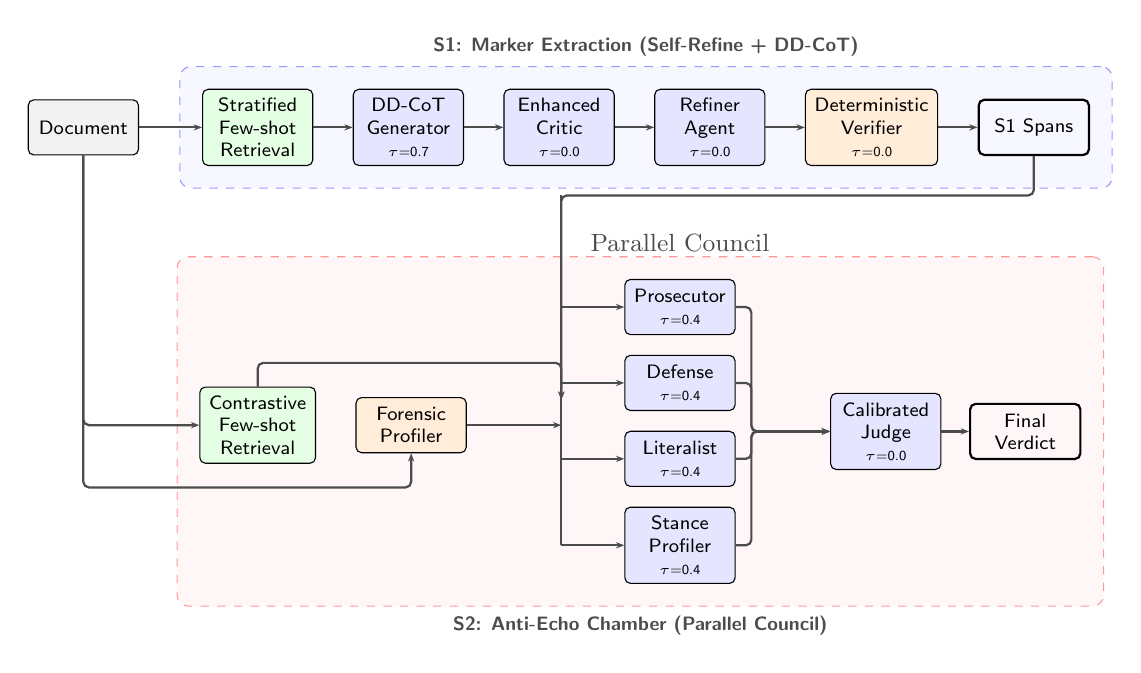
\begin{tikzpicture}[
        node distance=0.6cm and 0.4cm,
        >={Stealth[length=3pt]},
        inputbox/.style={rectangle, draw, rounded corners=2pt, minimum height=0.7cm,
                minimum width=1.4cm, align=center, font=\scriptsize\sffamily, fill=gray!10},
        ragbox/.style={rectangle, draw, rounded corners=2pt, minimum height=0.7cm,
                minimum width=1.4cm, align=center, font=\scriptsize\sffamily, fill=green!10},
        llmbox/.style={rectangle, draw, rounded corners=2pt, minimum height=0.7cm,
                minimum width=1.4cm, align=center, font=\scriptsize\sffamily, fill=blue!10},
        detbox/.style={rectangle, draw, rounded corners=2pt, minimum height=0.7cm,
                minimum width=1.4cm, align=center, font=\scriptsize\sffamily, fill=orange!15},
        outputbox/.style={rectangle, draw, rounded corners=2pt, minimum height=0.7cm,
                minimum width=1.4cm, align=center, font=\scriptsize\sffamily, thick},
        arrow/.style={->, thick, black!70, rounded corners=2pt}, line/.style={-, thick,
                black!70, rounded corners=2pt},
        grouplab/.style={font=\bfseries\scriptsize\sffamily, text=black!70}, ]

        % === INPUT ===
        \node[inputbox] (input) {Document};

        % === S1 PIPELINE (Top Row) ===
        \node[ragbox, right=0.8cm of input] (s1rag) {Stratified\\Few-shot\\Retrieval};
        \node[llmbox, right=0.5cm of s1rag] (gen) {DD-CoT\\Generator\\{\tiny $\tau$=0.7}};
        \node[llmbox, right=0.5cm of gen] (critic) {Enhanced\\Critic\\{\tiny $\tau$=0.0}};
        \node[llmbox, right=0.5cm of critic] (refiner) {Refiner\\Agent\\{\tiny $\tau$=0.0}};
        \node[detbox, right=0.5cm of refiner] (verifier) {Deterministic\\Verifier\\{\tiny $\tau$=0.0}};
        \node[outputbox, right=0.5cm of verifier] (s1out) {S1 Spans};

        % S1 Connections
        \draw[arrow] (input) -- (s1rag);
        \draw[arrow] (s1rag) -- (gen);
        \draw[arrow] (gen) -- (critic);
        \draw[arrow] (critic) -- (refiner);
        \draw[arrow] (refiner) -- (verifier);
        \draw[arrow] (verifier) -- (s1out);

        % S1 Group Box
        \begin{scope}[on background layer]
            \node[draw=blue!40, fill=blue!3, rounded corners=4pt, dashed,
            fit=(s1rag)(gen)(critic)(refiner)(verifier)(s1out),
            inner sep=8pt, label={[grouplab]above:{S1: Marker Extraction (Self-Refine + DD-CoT)}}] (s1group) {};
        \end{scope}

        % === S2 PIPELINE (Bottom Row) ===
        \node[ragbox, below=2.8cm of s1rag] (s2rag) {Contrastive\\Few-shot\\Retrieval};
        \node[detbox, right=0.5cm of s2rag] (forensic) {Forensic\\Profiler};

        % Parallel Council (Vertical Stack)
        \node[llmbox, right=2.0cm of forensic, yshift=1.5cm] (pros) {Prosecutor\\{\tiny $\tau$=0.4}};
        \node[llmbox, below=0.25cm of pros] (defense) {Defense\\{\tiny $\tau$=0.4}};
        \node[llmbox, below=0.25cm of defense] (literal) {Literalist\\{\tiny $\tau$=0.4}};
        \node[llmbox, below=0.25cm of literal] (stance) {Stance\\Profiler\\{\tiny $\tau$=0.4}};

        % Parallel Council Group Box
        \begin{scope}[on background layer]
            \node[draw=blue!40, fill=blue!3, rounded corners=3pt, dashed,
            fit=(pros)(defense)(literal)(stance),
            inner sep=6pt, label={[grouplab, font=\small]above:{Parallel Council}}] (pcgroup) {};
        \end{scope}

        % Judge & Verdict
        \coordinate (council_center) at ($(pros.north)!0.5!(stance.south)$);
        \node[llmbox, right=1.2cm of council_center -| stance.east] (judge) {Calibrated\\Judge\\{\tiny $\tau$=0.0}};
        \node[outputbox, right=0.35cm of judge] (verdict) {Final\\Verdict};

        % === WIRING THE BUS ===
        \coordinate (spine_x) at ($(forensic.east)!0.6!(defense.west)$);
        \coordinate (spine_top) at (spine_x |- s1out.south);
        \coordinate (spine_bot) at (spine_x |- stance.west);
        \draw[line] ($(spine_top) + (0, -0.5)$) -- (spine_bot);

        \draw[arrow] (s1out.south) -- ++(0,-0.5) -| (spine_x);
        \draw[arrow] (forensic.east) -- (forensic.east -| spine_x);
        \draw[arrow] (s2rag.north) -- ++(0,0.3) -| (spine_x);
        \draw[arrow] (input.south) |- (s2rag.west);
        \draw[arrow] (input.south) |- ($(s2rag.south) + (0,-0.3)$) -| (forensic.south);

        \foreach \agent in {pros, defense, literal, stance} {
                \draw[arrow] (spine_x |- \agent.west) -- (\agent.west);
            }
        \foreach \agent in {pros, defense, literal, stance} {
                \draw[arrow] (\agent.east) -- ++(0.2,0) |- (judge.west);
            }
        \draw[arrow] (judge) -- (verdict);

        % S2 Group Box
        \begin{scope}[on background layer]
            \node[draw=red!40, fill=red!3, rounded corners=4pt, dashed,
            fit=(s2rag)(forensic)(pros)(stance)(judge)(verdict),
            inner sep=8pt, label={[grouplab]below:{S2: Anti-Echo Chamber (Parallel Council)}}] (s2group) {};
        \end{scope}
    \end{tikzpicture}
    \end{center}
\end{frame}

% --- Slide 7: Tech Stack ---
\begin{frame}{Implementation: LangGraph \& PydanticAI Workflow}
    % Notice we removed [shrink] from the frame definition above
    
    \begin{center}
    % \resizebox scales the diagram to exactly 95% of the slide width
    \resizebox{0.55\textwidth}{!}{%
    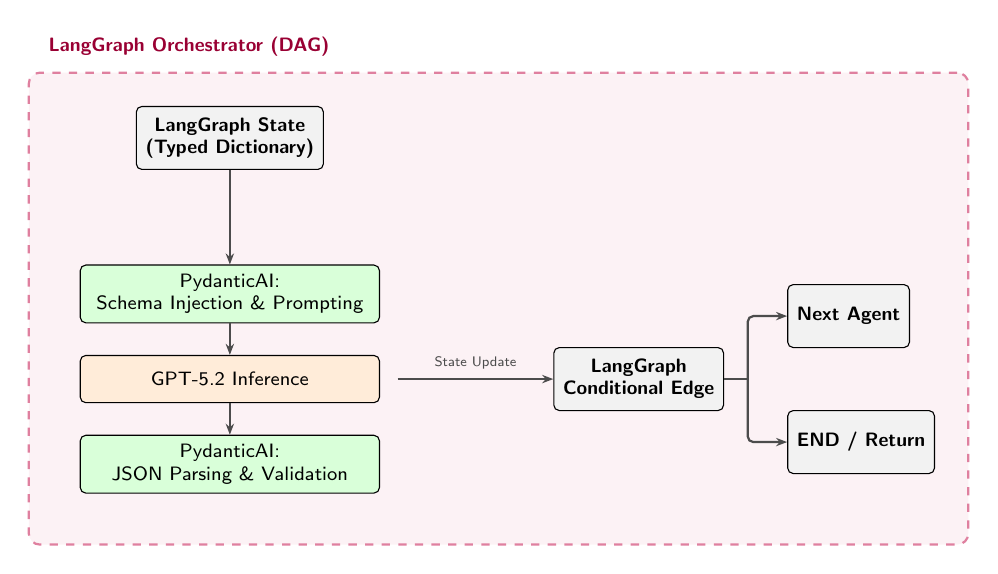
\begin{tikzpicture}[
        node distance=0.5cm and 0.8cm,
        >={Stealth[length=4pt, width=3pt]},
        groupbox/.style={rectangle, draw, rounded corners=4pt, dashed, thick},
        langgraph/.style={groupbox, fill=purple!5, draw=purple!50},
        agentbox/.style={groupbox, fill=blue!5, draw=blue!40},
        statebox/.style={rectangle, draw, rounded corners=2pt, fill=gray!10, minimum height=0.8cm, align=center, font=\scriptsize\sffamily\bfseries},
        pydantic/.style={rectangle, draw, rounded corners=2pt, fill=green!15, minimum width=3.8cm, minimum height=0.6cm, font=\scriptsize\sffamily, align=center},
        llm/.style={rectangle, draw, rounded corners=2pt, fill=orange!15, minimum width=3.8cm, minimum height=0.6cm, font=\scriptsize\sffamily, align=center},
        arrow/.style={->, thick, black!70, rounded corners=2pt},
        line/.style={-, thick, black!70, rounded corners=2pt},
        labelnode/.style={font=\scriptsize\sffamily\bfseries, text=black!80}
    ]

    % --- Core Nodes ---
    \node[statebox] (state_in) {LangGraph State\\(Typed Dictionary)};
    \node[pydantic, below=1.2cm of state_in] (schema_in) {PydanticAI:\\Schema Injection \& Prompting};
    \node[llm, below=0.4cm of schema_in] (model) {GPT-5.2 Inference};
    \node[pydantic, below=0.4cm of model] (schema_out) {PydanticAI:\\JSON Parsing \& Validation};

    \node[statebox, right=2.2cm of model] (router) {LangGraph\\Conditional Edge};
    \node[statebox, right=0.8cm of router, yshift=0.8cm] (next_agent) {Next Agent};
    \node[statebox, right=0.8cm of router, yshift=-0.8cm] (end) {END / Return};

    % --- Grouping Boxes (Background Layer) ---
    \begin{scope}[on background layer]
        % Agent Box
        \node[agentbox, fit=(schema_in)(model)(schema_out), inner sep=6pt] (agent) {};
        % Explicitly placed label prevents parsing errors
        \node[labelnode, anchor=south, yshift=2pt] at (agent.north) {Agent Node Execution};

        % LangGraph Box
        \node[langgraph, fit=(state_in)(agent)(router)(next_agent)(end), inner sep=12pt] (lg) {};
        \node[labelnode, text=purple!80!black, anchor=south west, xshift=4pt, yshift=2pt] at (lg.north west) {LangGraph Orchestrator (DAG)};
    \end{scope}

    % --- Connections ---
    \draw[arrow] (state_in.south) -- (schema_in.north);
    \draw[arrow] (schema_in.south) -- (model.north);
    \draw[arrow] (model.south) -- (schema_out.north);

    % Arrow from the right edge of the Agent box to the Router
    \draw[arrow] (agent.east |- router.west) -- node[above, font=\tiny\sffamily] {State Update} (router.west);

    % Routing Branching
    \draw[line] (router.east) -- ++(0.3,0) coordinate (fork);
    \draw[arrow] (fork) |- (next_agent.west);
    \draw[arrow] (fork) |- (end.west);

    \end{tikzpicture}%
    } % <-- Closes the resizebox
    \end{center}
    
    
    \begin{itemize}
        \item \textbf{LangGraph Orchestration:} Maintains the global typed state across the pipeline and handles directed acyclic graph (DAG) routing between distinct personas.
        \item \textbf{PydanticAI Enforcement:} Sits inside each LangGraph node. It translates Python data models into strict JSON constraints for GPT-5.2, guaranteeing that intermediate artifacts (critiques, votes) are parseable.
    \end{itemize}
\end{frame}

% --- Slide 8: Multi-Agent Paradigms ---
\begin{frame}{Applied Agentic Paradigms (LangGraph)}
    \small We structured our system around two foundational patterns to solve specific LLM failure modes:
    \vspace{0.2cm}
    
    \begin{columns}[T]
        % --- Left Column: Evaluator-Optimizer (S1) ---
        \begin{column}{0.48\textwidth}
            \centering
            
            \includegraphics[width=\linewidth]{images/evaluator_optimizer.png} 
            \vspace{0.1cm}
            
            \raggedright
            \textbf{1. Evaluator-Optimizer (S1)}
            \scriptsize
            \setlength{\leftmargini}{1.2em} % Safe way to reduce left margin in Beamer
            \begin{itemize}
                \item \textbf{Pattern:} Iterative refinement (Draft $\rightarrow$ Audit $\rightarrow$ Edit).
                \item \textbf{Purpose:} Single-pass LLMs fail at exact character boundaries. Iteration is required for structural precision.
            \end{itemize}
        \end{column}
        
        % --- Right Column: Parallelization (S2) ---
        \begin{column}{0.48\textwidth}
            \centering
            
            \includegraphics[width=\linewidth]{images/orchestrator_worker.png} 
            \vspace{0.1cm}
            
            \raggedright
            \textbf{2. Parallelization / Voting (S2)}
            \scriptsize
            \setlength{\leftmargini}{1.2em} % Safe way to reduce left margin in Beamer
            \begin{itemize}
                \item \textbf{Pattern:} Concurrent evaluation $\rightarrow$ Aggregation.
                \item \textbf{Purpose:} Sequential prompting causes "groupthink". Parallelization enforces diverse, adversarial viewpoints.
            \end{itemize}
        \end{column}
    \end{columns}
\end{frame}

% --- Slide 8: S1 Mechanism ---
\begin{frame}{S1: Marker Extraction via DD-CoT \& Self-Refine}
    
    \begin{itemize}
        \item \textbf{Dynamic Discriminative Chain-of-Thought (DD-CoT):} The generator must explicitly state evidence for a label AND a counter-argument against confusable alternative labels. 
        \item \textbf{Self-Refine Loop:} Standard critique-revise pattern applied to typed artifacts.
        \begin{itemize}
            \item \textit{Generator:} Proposes labeled marker strings.
            \item \textit{Critic:} Checks verbatimness, label discrimination, and hallucinatory spans.
            \item \textit{Refiner:} Applies surgical, minimal edits based on the critique.
        \end{itemize}
        \item \textbf{Deterministic Verifier:} Maps strings to exact character offsets via a matching cascade, avoiding "hallucinated spans".
    \end{itemize}
\end{frame}

% --- Slide 9: S2 Mechanism ---
\begin{frame}{S2: Conspiracy Detection via Anti-Echo Chamber}
    
    \begin{itemize}
        \item \textbf{The Reporter Trap:} The baseline model's failure mode where topical discussion or neutral reporting of conspiracies is conflated with endorsement.
        \item \textbf{The Parallel Council:} Four independent personas deliberate simultaneously:
        \begin{itemize}
            \item \textit{Prosecutor:} Identifies evidence for conspiracy endorsement.
            \item \textit{Defense Attorney:} Presents exculpatory evidence against endorsement.
            \item \textit{Literalist:} Independently checks literal entailment.
            \item \textit{Stance Profiler:} Analyzes certainty and group dynamics.
        \end{itemize}
        \item \textbf{Calibrated Judge:} Aggregates votes with conservative confidence rules, defaulting to non-conspiracy when ambiguous.
    \end{itemize}
\end{frame}

% --- Slide 10a: Knowledge Base Construction (Offline) ---
\begin{frame}{Knowledge Base Construction: Ingestion \& Enrichment}
    \small Before deploying our agents, we construct a high-quality, persistent few-shot memory bank to enable robust in-context learning.
    
    \vspace{0.2cm}
    
    \begin{columns}[T, onlytextwidth]
        \begin{column}{0.48\textwidth}
            \textbf{1. Diverse Sampling (MMR)}
            \begin{itemize}
                \scriptsize % Reduced from \footnotesize to save vertical space
                \setlength{\itemsep}{0.2em} % Tighter line spacing
                \item \textbf{Objective:} Maximize linguistic coverage while eliminating redundancy.
                \item \textbf{Implementation:} Applied Maximal Marginal Relevance (MMR) via OpenAI \texttt{text-embedding-3-small}.
                \item \textbf{Scale:} Filters dataset to a maximally diverse core of $\sim$500 documents per subtask.
            \end{itemize}
        \end{column}
        
        \begin{column}{0.48\textwidth}
            \textbf{2. Teacher Agent Rationales}
            \begin{itemize}
                \scriptsize % Reduced from \footnotesize to save vertical space
                \setlength{\itemsep}{0.2em} % Tighter line spacing
                \item \textbf{Objective:} Provide inference LLMs with explicit ``how to think'' reasoning chains.
                \item \textbf{Implementation:} Specialized personas (e.g., \textit{Supreme Court Justice} for S2) analyze the MMR subset.
                \item \textbf{Storage:} Enriched documents and metadata are persistently indexed in \textbf{ChromaDB}.
            \end{itemize}
        \end{column}
    \end{columns}
        
    % Replaced the bulky alertblock with a sleek, space-saving alternative
    \rule{\textwidth}{0.1pt}
    
    \textbf{\textcolor{ailsred}{Contrastive In-Context Learning Transition:}} \\
    \footnotesize At inference time, we do \textbf{not} perform standard RAG (fact augmentation). Instead, we query ChromaDB to dynamically fetch \textbf{discriminative few-shot examples}, teaching the model how to handle semantic boundary cases on the fly.
\end{frame}

% --- Slide 10: Contrastive Retrieval ---
\begin{frame}{Contrastive Few-Shot Retrieval}
    \begin{columns}
        \begin{column}{0.48\textwidth}
            \begin{itemize}
                \item \textbf{S1 Stratified Sampling:} Allocates 60\% retrieval weight to underrepresented categories (e.g., EVIDENCE) to ensure balanced prompt exposure.
                \item \textbf{S2 Hard Negatives:} Mines non-conspiracy documents that still contain S1 marker vocabulary. 
                \item Forces the S2 council to attend to hedging and attribution rather than simple topical overlap.
                \item \textbf{Reranking:} BAAI cross-encoder prioritizes structural similarities.
            \end{itemize}
        \end{column}
        \begin{column}{0.5\textwidth}
            \resizebox{\linewidth}{!}{
            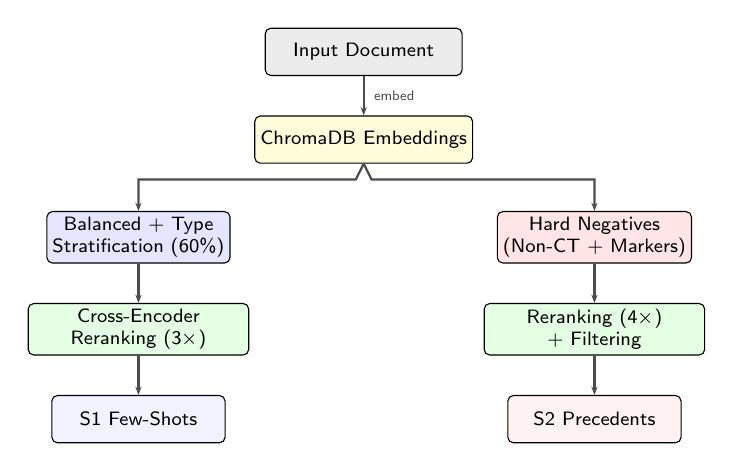
\begin{tikzpicture}[
                node distance=0.5cm and 0.4cm,
                >={Stealth[length=3pt]},
                box/.style={rectangle, draw, rounded corners=2pt, minimum height=0.6cm,
                        align=center, font=\scriptsize\sffamily, inner sep=2pt},
                sbox/.style={box, fill=blue!10, minimum width=2.2cm},
                nbox/.style={box, fill=red!10, minimum width=2.2cm},
                gbox/.style={box, fill=green!10, minimum width=2.8cm},
                arrow/.style={->, thick, black!70},
                ]

                \node[box, fill=gray!15, minimum width=2.5cm] (query) {Input Document};
                \node[box, fill=yellow!15, below=0.5cm of query, minimum width=2.5cm] (chroma) {ChromaDB Embeddings};
                \draw[arrow] (query) -- node[right, font=\tiny\sffamily] {embed} (chroma);

                \node[sbox, below left=0.6cm and 0.3cm of chroma] (s1ret) {Balanced + Type\\Stratification (60\%)};
                \node[nbox, below right=0.6cm and 0.3cm of chroma] (s2ret) {Hard Negatives\\(Non-CT + Markers)};
                \draw[arrow] (chroma.south) -- ++(-0.1,-0.2) -| (s1ret.north);
                \draw[arrow] (chroma.south) -- ++(0.1,-0.2) -| (s2ret.north);

                \node[gbox, below=0.5cm of s1ret] (rerank1) {Cross-Encoder\\Reranking (3×)};
                \node[gbox, below=0.5cm of s2ret] (rerank2) {Reranking (4×)\\+ Filtering};
                \draw[arrow] (s1ret) -- (rerank1);
                \draw[arrow] (s2ret) -- (rerank2);

                \node[box, fill=blue!5, below=0.5cm of rerank1, minimum width=2.2cm] (out1) {S1 Few-Shots};
                \node[box, fill=red!5, below=0.5cm of rerank2, minimum width=2.2cm] (out2) {S2 Precedents};
                \draw[arrow] (rerank1) -- (out1);
                \draw[arrow] (rerank2) -- (out2);
            \end{tikzpicture}
            }
        \end{column}
    \end{columns}
\end{frame}

% --- Slide 11: Prompt Optimization ---
\begin{frame}{Prompt Optimization: GEPA with MLflow}
    \begin{columns}
        \begin{column}{0.48\textwidth}
            \begin{itemize}
                \item Evolves prompts using Genetic Evolution Prompt Algorithm (GEPA) in MLflow.
                \item \textbf{Crossover:} Merges complementary elements of successful parents.
                \item \textbf{Reflective LLM Mutation:} Uses GPT-5.2 to propose targeted edits based on aggregated error logs.
                \item \textbf{Fitness Metrics:} 
                \begin{itemize}
                    \item S1: Macro $F_2$
                    \item S2: Gradient Consensus
                \end{itemize}
            \end{itemize}
        \end{column}
        \begin{column}{0.5\textwidth}
            \resizebox{\linewidth}{!}{
            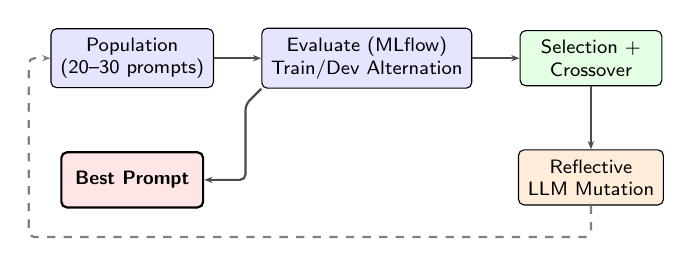
\begin{tikzpicture}[
                node distance=0.6cm and 0.5cm,
                >={Stealth[length=3pt]},
                process/.style={rectangle, draw, rounded corners=2pt, minimum height=0.7cm,
                        minimum width=1.8cm, align=center, font=\scriptsize\sffamily, fill=blue!10},
                decision/.style={rectangle, draw, rounded corners=2pt, minimum height=0.7cm,
                        minimum width=1.8cm, align=center, font=\scriptsize\sffamily, fill=green!10},
                mutation/.style={rectangle, draw, rounded corners=2pt, minimum height=0.7cm,
                        minimum width=1.8cm, align=center, font=\scriptsize\sffamily, fill=orange!15},
                output/.style={rectangle, draw, rounded corners=2pt, minimum height=0.7cm,
                        minimum width=1.8cm, align=center, font=\bfseries\scriptsize\sffamily,
                        fill=red!10, thick},
                arrow/.style={->, thick, black!70, rounded corners=2pt},
                dasharrow/.style={->, thick, dashed, black!50, rounded corners=2pt},
                ]

                \node[process] (pop) {Population\\(20--30 prompts)};
                \node[process, right=0.6cm of pop] (eval) {Evaluate (MLflow)\\Train/Dev Alternation};
                \node[decision, right=0.6cm of eval] (select) {Selection +\\Crossover};
                \node[mutation, below=0.8cm of select] (mutate) {Reflective\\LLM Mutation};
                \node[output, below=0.8cm of pop] (best) {Best Prompt};

                \draw[arrow] (pop) -- (eval);
                \draw[arrow] (eval) -- (select);
                \draw[arrow] (select) -- (mutate);

                \draw[dasharrow] (mutate.south) -- ++(0,-0.4)
                -| ([xshift=-0.4cm]best.west)
                |- (pop.west);
                \draw[arrow] (eval.south west) -- ++(-0.2,-0.2) |- (best.east);
            \end{tikzpicture}
            }
        \end{column}
    \end{columns}
\end{frame}

% ==========================================
\section{3. Results \& Evaluation}
% ==========================================

% --- Slide 12: Experimental Setup ---
\begin{frame}{Experimental Setup \& LLMOps}
    \vspace{0.2cm}
    \begin{itemize}
        \item \textbf{Data Splits:} Followed official SemEval train/dev/test splits (100 documents for dev, 938 for test).
        \item \textbf{Baseline:} Zero-shot GPT-5.2 classifier/extractor using a single, static prompt.
        \item \textbf{Experiment Tracking (MLflow):} All agentic traces, prompt mutations, and evaluation metrics were rigorously logged. This LLMOps integration ensured full reproducibility across our complex LangGraph workflows.
        \item \textbf{Temperature Stratification:} 
        \begin{itemize}
            \item $\tau=0.7$ for the DD-CoT Generator (encourages candidate exploration).
            \item $\tau=0.4$ for Council Jurors (balances diverse reasoning with consistent verdicts).
            \item $\tau=0.0$ for Critic, Refiner, and Judge (ensures deterministic reproducibility).
        \end{itemize}
    \end{itemize}
\end{frame}

% --- Slide 13: Results & Findings ---
\begin{frame}{Results \& Findings}
    \begin{itemize}
        \item \textbf{Major Improvements:} The agentic pipeline doubled extraction (S1) performance and dramatically improved classification (S2) on the Dev set.
        \item \textbf{Official SemEval Standings:}
        \begin{itemize}
            \item \textbf{Subtask 1:} Ranked \textbf{Top 10} globally on the Test set (trailing 1st place by just $0.04$ Macro $F_1$), and \textbf{Top 3} on the Dev set .
            \item \textbf{Subtask 2:} Ranked \textbf{Top 5} on the Dev set and \textbf{Top 20} globally on the Test set.
        \end{itemize}
    \end{itemize}
    
    \vspace{0.2cm}
    
    \begin{table}[h]
        \centering
        \normalsize % Adjusted to give the text above more room
        \begin{tabular}{llrrr}
        \toprule
        \textbf{Task \& Metric} & \textbf{Split} & \textbf{Baseline} & \textbf{Agentic} & \textbf{$\Delta$} \\ \midrule
        \multirow{2}{*}{\textbf{S1} (Macro $F_1$)} & Dev (100)  & 0.12 & \textcolor{blue}{\textbf{0.24}} & +100\% \\
                            & Test (938) & --   & 0.21 & -- \\ \midrule
        \multirow{2}{*}{\textbf{S2} (Weighted $F_1$)} & Dev (100)  & 0.53 & \textcolor{blue}{\textbf{0.79}} & +49\% \\
                            & Test (938) & --   & 0.75 & -- \\ \bottomrule
        \end{tabular}
    \end{table}
\end{frame}

% --- Slide 14: Qualitative Analysis ---
\begin{frame}{Qualitative Analysis: System in Action}
    
    \begin{itemize}
        \item \textbf{Agency Disentanglement (S1):} The baseline frequently mistakes grammatical subjects for semantic agents (subject-position bias). Our DD-CoT correctly reassigns passive subjects to \textsc{Victim} and identifies the true \textsc{Actor}.
        \item \textbf{Reporter Trap Mitigation (S2):} The baseline flags neutral reporting as endorsement. Our Anti-Echo Chamber utilizes the Defense Attorney to parse attribution verbs (e.g., \textit{"claims"}), classifying it accurately.
    \end{itemize}
    \vspace{0.3cm}
    \begin{table}[h]
        \centering
        \small
        \begin{tabular}{@{}p{5cm}p{3cm}p{4cm}@{}}
            \toprule
            \textbf{Text Snippet} & \textbf{Baseline} & \textbf{Our System (Agentic)} \\
            \midrule
            \textit{``The public was manipulated by the media...''} & \textsc{Actor}: The public & \textsc{Actor}: the media \newline \textsc{Victim}: The public \\
            \midrule
            \textit{``The article claims that the earth is flat.''} & Endorsement & Neutral Reporting \\
            \bottomrule
        \end{tabular}
    \end{table}
\end{frame}

% --- Slide 15: Ablation Studies ---
\begin{frame}{Ablation Studies}
    \begin{itemize}
        \item \textbf{Self-Refine} yields the largest single S1 gain by correcting boundaries.
        \item \textbf{Contrastive Retrieval} directly halves the S2 false-positive rate.
        \item A ``Leave-One-Out'' analysis confirmed that removing the \textbf{Prosecutor} drops $F_1$ heavily (loss of signal), while removing skeptical jurors degrades precision.
    \end{itemize}
    \vspace{0.2cm}
    \begin{table}[h]
        \centering
        \small
        \begin{tabular}{cllrrr}
        \toprule
        & \textbf{Component / Change} & \textbf{Metric} & \textbf{Base} & \textbf{Agentic} & \textbf{$\Delta$} \\ \midrule
        \multirow{2}{*}{S1} & \textbf{Self-Refine} (Audit loop) & Macro F1 & 0.173 & 0.240 & +0.067 \\
        & \textbf{DD-CoT} (Perpetrator vs Victim) & Actor F1 & 0.263 & 0.290 & +0.027 \\ \midrule
        \multirow{3}{*}{S2} & \textbf{Parallel Council} (Debate) & Recall & 0.481 & 0.560 & +0.079 \\
        & \textbf{Prosecutor} (Evidence for) & F1 Score & 0.680 & 0.795 & +0.115 \\
        & \textbf{Contrastive Retrieval} (Hard Negs) & FP Rate & 0.160 & 0.080 & $-$0.080 \\
        \bottomrule
        \end{tabular}
    \end{table}
\end{frame}

% --- Slide 16: The Compute-Accuracy Trade-off ---
\begin{frame}{The Compute-Accuracy Trade-off}
    \begin{itemize}
        \item \textbf{Deliberate Architectural Choice:} We explicitly exchange inference-time compute for superior zero-shot performance and structural precision.
        \item \textbf{Overhead vs. Scaling:} The agentic workflow necessitates $\sim$4x to 5x more LLM calls per document compared to a single-pass baseline.
        \item Crucially, latency scales linearly with document length but remains predictable per document.
    \end{itemize}
    \vspace{0.2cm}
    \begin{table}[h]
        \centering
        \normalsize
        \begin{tabular}{llrrr}
        \toprule
        \textbf{Stage} & \textbf{Configuration} & \textbf{Latency (s)} & \textbf{Tokens} & \textbf{Calls} \\ \midrule
        \multirow{2}{*}{S1} & Baseline (Generator only) & 10.5 & 2{,}549 & 1.0 \\
                            & Full Graph (Self-Refine)   & 30.2 & 7{,}986 & 2.5 \\ \midrule
        \multirow{2}{*}{S2} & Baseline (Single Agent)       & 4.6  & 1{,}665 & 1.0 \\
                            & Full Graph (Council + Judge)   & 29.1 & 12{,}627 & 5.0 \\ \bottomrule
        \end{tabular}
    \end{table}
\end{frame}

% --- Slide 17: Portability to Open-Weights Models ---
\begin{frame}{Portability to Open-Weights Models}
    \begin{itemize}
        \item We evaluated a smaller, open-weights model, Qwen-3-8B-Instruct, to test architectural portability.
        \item \textbf{Scientific Insight:} Strict JSON schema enforcement and complex discriminative reasoning (DD-CoT) are \textbf{emergent capabilities of frontier models}.
        \item \textbf{The Adaptation:} Smaller models require \emph{relaxed constraints} rather than exhibiting outright failure. We deployed a \textbf{Lite S1 Agent} (simplified 3-field schema) and a \textbf{Dyadic Debate S2} (Prosecutor vs. Defense).
        \item \textbf{Results:} Achieved 0.16 Macro $F_1$ on S1 and 0.63 Weighted $F_1$ on S2.
        \item \textbf{Takeaway:} Core agentic reasoning transfers meaningfully to open-weights models when the workflow is appropriately calibrated to their schema-following capacity.
    \end{itemize}
\end{frame}

% --- Slide 18: Conclusion ---
\begin{frame}{Conclusion}
    \begin{itemize}
        \item \textbf{Workflow Replaces Scaling:} This work demonstrates that deliberate workflow structure can effectively substitute for model scaling or data curation.
        \item \textbf{Decoupling is Key:} Decoupling semantic reasoning from deterministic span localization doubles baseline extraction performance by resolving character-level brittleness.
        \item \textbf{Defeating the Reporter Trap:} A Parallel Council and Calibrated Judge, paired with contrastive retrieval, successfully suppress false positives.
    \end{itemize}
\end{frame}

% --- Slide 19: Limitations & Future Research ---
\begin{frame}{Critical Reflection: Limitations \& Future Work}
    \begin{columns}[T]
        \begin{column}{0.48\textwidth}
            \textbf{Current Limitations}
            \begin{itemize}
                \scriptsize
                \setlength{\itemsep}{0.4em}
                \item \textbf{Inference Overhead:} Agentic workflows require $\sim$5x more calls and thus increased latency, impacting real-time deployment.
                \item \textbf{Hardware Constraints:} Fine-tuning open-source models (like Qwen-3-8B) was limited by available GPU VRAM.
                \item \textbf{Schema Brittleness:} Smaller models struggle with strict PydanticAI JSON enforcement.
            \end{itemize}
        \end{column}
        
        \begin{column}{0.48\textwidth}
            \textbf{Future Directions}
            \begin{itemize}
                \scriptsize
                \setlength{\itemsep}{0.4em}
                \item \textbf{Heterogeneous LLM Routing:} Using \textbf{LiteLLM} to route tasks by complexity:
                \begin{itemize}
                    \tiny
                    \item \textit{Premium Models} (GPT-5.2, Opus) for initial generation.
                    \item \textit{Efficient Models} (Gemini Flash, GPT-5 mini) for Council/Critic roles.
                \end{itemize}
                \item \textbf{Agentic Distillation:} Fine-tuning GLM/MiniMax/Qwen on agentic traces to create high-performance specialized "single-pass" models.
            \end{itemize}
        \end{column}
    \end{columns}
\end{frame}

\begin{frame}[standout]
    Thank You \\
    \vspace{1em}
    \normalsize Questions?
\end{frame}

\end{document}